\chapter{بررسی کارهای مرتبط}
\section{بررسی مرجع \cite{hawthorne2017onsets}}
در این مقاله با استفاده از شبکه‌های عصبی پیچشی و شبکه‌های عصبی بازگشتی که به صورت
همراه آموزش داده شده بودند تا اطلاعات شروع نت و نت‌های فعال در هر فرم را تشخصی
دهند، موفق شدند تا رشدی بیش از ۱۰۰ درصد در دقت نسبی مسئله ایجاد کنند. این مدل
ابتدا فشرده شدن هر نت را تشخیص می‌دهد و سپس با استفاده از این اطلاعات، نت‌های
موجود در هر فرم زمانی را تشخیص می‌دهند. در زمان استنداج نت‌های پیشبینی شده در هر
فرم زمانی تنها در صورتی معتبر شناخته می‌شود که قبل‌تر مدل شروع یک نت را تشخیص
داده باشد. این مقاله تلاش کرده است که هر دوی معیارهای شروع نت و طول نت فعال را
با هم افزایش دهد که با توجه نوع درک ما از موسیقی، انتخابی مناسب‌تر از افزایش
جداگونه این معیارها هست. در نهایت این مدل با اضافه کردن معیاری جدید، شدت هر نت
هم پیشبینی کرده است که موجب به آوانوسی طبیعی‌تر می‌شود.

\subsection{دیتاست و معیارها}
برای آموزش مدل از دیتاست
MAPS
استفاده شده است که شامل هم قطعات تولید شده با استفاده از نرم‌افزار هم قطعات ضبط
شده از یک پیانو واقعی است. قطعات ساختگی برای آموزش مدل و قطعات ضبط شده برای فاز
استنداج استفاده شده است. همچنین اطمینان حاصل شده است که هر قطعه فقط در یکی از
بخش‌های دیتا وجود داشته باشد. همچنان استفاده از قطعات ضبط شده برای استناج و بررسی
دقت مدل واقعگرایانه‌تر است زیرا اغب از آوانویسی موسیقی رو بر روی قطعات ضبط شده
از پیانوی واقعی استفاده می‌شود.

در پیش‌پردازش ابتدایی دیتا فعال بودن پدال نگهدارنده پیانو به طول بیشتر نت‌ها
تبدیل شده است. در صورتی که نتی در زمان فعال بودن پدال نگهدارنده فشرده شود، نت
تا پایان فعال بودن پدال یا مجددا فشرده شدن همان نت، کشیده می‌شود. این پروسه
باعث می‌شود که مدل نیازی به درک پدال نگهدارنده نداشته باشد و بتوان مدل یکسانی
برای سازی دیگر استفاده شود.

معیارهای استفاده برای ارزیابی مدل هم بر اساس فرم و هم بر اساس نت هستند و شامل
دقت، فراخوانی و 
f1
می‌باشند. برای پیاده‌سازی این معیارها از کتاب‌خانه
\lr{mir eval} \cite{raffel2014mir_eval}
استفاده شده است. دو نسخه برای هر یک از معیارها استفاده شده است. برای نسخه اول
تنها لازم هست که شروع هر نت در فاصله ۵۰ میلی‌ثانیه‌ای زمان حقیقی باشد. ولی بر روی
طول هر نت محدودیتی وجود نداره. نسخه دوم علاوه بر پیشنیاز قبلی نیازدارد تا طول هر
نت در بیشنیه ۲۰ درصدی مقدار واقعی و فاصله ۵۰ میلی‌ثانیه‌ای مقدار واقعی باشد.
همچنین یک معیار جدید برای یک معیار جدید برای اندازه گیری شدت هر نت معرفی شده
است. تمام معیارها برای هر قطعه جدا حساب شده‌اند و میانگین به عنوان نتیجه نهایی
گزارش شده است.

\subsection{تنظیمات مدل}
مدل‌های معرفی شده قبلی فرض می‌کردند که تمام فرم‌ها ارزشی یکسان دارند و از هم
مستقل‌اند. این مقاله معتقد است که بعضی از فرم‌ها ارزش بیشتری نسبت به سایر فرم‌ها
دارند. به صورت دقیق‌تر فرم‌هایی که نتی در آن‌ها شروع می‌شود پراهمیت‌تر از سایر فرم‌ها
هستند. از آن‌جا که شدت صدای هر نت پیانو بلافاصله پس از فعال شدن شروع به افت می‌کند،
پس فرم اول هر نت هم ساده‌ترین فرم برای تشخصی آن نت است و هم اهمیت شنیداری بسیار
بیشتری را دارد.

برای استفاده از این اهمیت یک بخش مدل فقط وظیفه تشخیص شروع نت‌ها را دارد و از این
خروجی این بخش در ادامه استفاده می‌شود تا فعال بودن نت در هر فرم را تشخیص دهد.
تنها در صورتی فرض می‌شود در یک فرم، نتی فعال است که فعال شدن آن در همان فرم یا
یک فرم قبلی تشخصی داده شده باشد.

تشخیص دهنده‌های شروع و فعال بودن نت‌ها بر پایه شبکه عصبی پیچشی معرفی شده در
\cite{kelz2016potential}
هستند با مقداری تغییر. هم چنین از کتاب‌خانه
\lr{librosa} \cite{mcfee2015librosa}
استفاده شده است تا از روی صوت ورودی نمایش
\lr{mel-scaled spectrograms}
آن محاسبه شود.

تشخیص دهنده شروع نت شامل یک شبکه عصبی پیچشی هستند که
خروجی آن‌ها به یک شبکه حافظه کوتاه مدت مانگار دوجهته داده می‌شود. در نهایت خروجی
این لایه به یک لایه تماما همبند داده می‌شود داده می‌شود که ۸۸ خروجی دارد و از تابع
فعال‌سازی
\lr{sigmoid}
استفاده می‌کند. هر کدام از این ۸۸ نرون خروجی نماینده یک کلاویه از پیانو هستند.

تشخیص دهنده فعال بودن هر نت یک از شبکه عصبی پیچشی دیگر تشکیل شده است که در
ادامه آن یک لایه تماما همبند با ۸۸ نرون خروجی قرار دارد. خروجی آن به خروجی
تشخیص دهنده شروع نت متصل می‌شود و به شبکه حافظه کوتاه مدت ماندگار دو جهته داده
می‌شود. در نهایت یک لایه تمام همبند دیگر با ۸۸ نرون خروجی و تابع فعال‌سازی
\lr{sigmoid}
قرار دارد.

\begin{figure}
    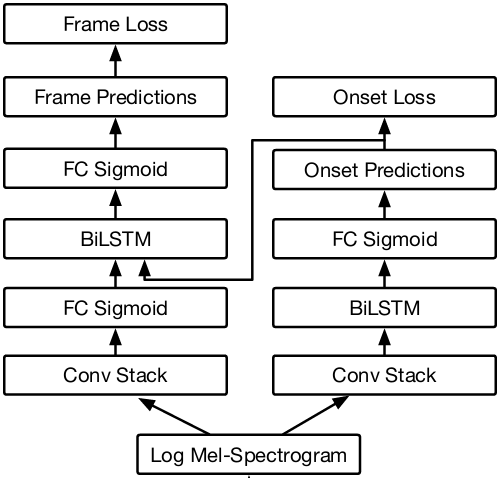
\includegraphics[width=\linewidth]
    {./statics/onset_onframe_network_architecture.png}
    \caption{ساختار شبکه استفاده شده}
\end{figure}

برای افزایش سرعت آموزش داده‌های آموزشی به فایل‌های کوچک‌تری تقسیم شده‌اند. همچنین
هرجای فایل برای این تقسیم کردن مناسب نمی‌باشد، زیرا در صورتی که شروع نت در فایل
قبلی قرار گیرد، تشخیص دهنده نت فعال نمی‌تواند ادامه نت‌ها را تشخصیص دهد. از این
جهت فایل‌ها به فواصل ۲۰ ثانیه تقسیم شده‌اند تا هم تعداد این نقاط شکستی زیاد نباشد
و هم بتوان از دسته‌هایی با اندازه حداقل ۸ استفاده کرد.

از آنجایی که فایل‌های صوتی به فرم‌های کوچک برای پرداز تقسیم می‌شود، پس برچسب‌ها هم
فرم بندی شوند. در زمان آموزش طول فرم برچسب‌ها و فایل صوتی برابر است. در هنگاه
محاسبه معایرهای دقت‌سنجی مدل، از زمان واقعی هر اتفاق استفاده می‌شود.

\subsection{تابع خطا}
تابع خطای استفاده شده در مدل مجموع دو تابع خطای دیگر
\lr{cross-entropy}
هست که یکی از آن‌ها مربوط به بخش تشخیص دهنده شروع نت و دیگری مطعلق به بخش تشخیص
دهده فعال بودن نت است.

\begin{equation}
    L_{total} = L_{onset} + L{frame}
\end{equation}

\begin{equation}
    L_{onset} = \sum_{p=p_{min}}^{p_{max}}\sum_{t=0}^{T}
    CE(I_{onset}(p, t), P_{onset}(p, t))
\end{equation}

در معادله بالا
$p_{min}$
و
$p_{max}$
نشان دهنده بازه نت‌ها هستند. همچنین
T
نشان‌دهنده تعداد فرم‌ها در یک نمونه آموزشی است.
$I_{onset}$
یک تابع هست که اگر نت
p
در زمان
t
فعال‌شده باشد، مقدار آن ۱ و در غیر این صورت ۰ است. همچنین
$P_{onset}$
احتمال فعال شدن نت
p
در زمان
t
است که توسط تشخیص دهنده فعال شدن نت محاسبه می‌شود. همچنین
CE
تابع
\lr{cross-entropy}
هست.

همچنین برای محاسبه
$L_{frame}$
رابطه زیر با تعاریف مشابه استفاده می‌شود.

\begin{equation}
    L_{frame} = \sum_{p=p_{min}}^{p_{max}}\sum_{t=0}^{T}
    CE(I_{frame}(p, t), P_{frame}(p, t))
\end{equation}

که در آن
$I_{frame}$
مقدار ۱ دارد اگر نت
p
در زمان
t
فعال باشد و ۰ دارد در صورتی که شرط برقرار نباشد. همچنین
$P_{frame}$
احتمالی هست که توسط تشخیص دهنده فعال بودن نت محاسبه می‌شود.

\subsection{تشخصیص شدت نواختن}
این مدل شامل یک شبکه دیگر نیز هست که وظیفه آن تقریب میزان شدت هر نت است. ساختار
این شبکه مشابه تشخیص دهنده فعال شدن نت است با این تفاوت که خروجی آن به بخش دیگری
از مدل داده نمی‌شود. همچنین برچسب‌های شدت از تقسیم مقدار شدت هر نت بر بیشینه شدت
نواخته شده در قطعه است. شدت کمترین نت در نتیجه ۰ نمی‌شود و برابر
$\frac{V_{min}}{V_{max}}$
است.

این بخش از مدل از تابع خطای زیر برای آموزش استفاده می‌کند:
\begin{equation}
    L_{vel} = \sum_{p=p_{min}}^{p_{max}}\sum_{t=0}^{T}
    I_{onset}(p, t)(v_{label}^{p,t} - v_{predicted}^{p, t})^2
\end{equation}

در زمان انستنتاج این شدت نسبی توسط رابطه زیر به شدت
MIDI
تبدیل می‌شود.
\begin{equation}
    v_{midi} = 80v_{predicted} + 10
\end{equation}

هرچند این مقدارها کاملا دلخواه هستند ولی صوت‌های ایجاد شده از این آوانوسی‌ها خروجی
لذت‌بخش داشته‌اند.

ارزیابی پیشبینی شدت هر نت کاری بدیهی محسوب نمی‌شود. زیرا برخلاف پیشبینی فعال شدن
یا فعال بودن یک نت در هر فرم، شدت هیچ معنای مطلقی ندارد. برای مثال دو قطعه کاملا
یکسان را در نظر بگیرد فقط با این تفاوت که شدت هر نت در یکی از قطعات برابر کسری
ثابت از شدت همان نت در قطعه دیگر باشد. در این صورت با وجود این که مقدار عددی
شدت‌ها متفاوت است ولی دو قعطه یکسان محسوب می‌شوند.

برای حل این مشکل ابتدا تمام شدت‌های موجود در یک قطعه بر بیشتر شدت قطعه تقسیم
می‌شوند تا در نتیجه تمام شدت‌ها در بازه
$[0,1]$
قرار گیرند. سپس اگر شدت‌های واقعی را 
$v_r$
و شدت‌های تخمین زده شده را
$v_e$
بنامیم، با استفاده از یک رگریوسن خطی دو پارامتر
m
و
b
را محسابه می‌کنیم که به ترتیب حکم شب و عرض از مبدا این تبدیل خطی را دارند.
\begin{equation}
    m, b = argmin_{m, b} \sum_{i=1}^{M}
    | v_r(i) - (mv_e(i) + b) |^2
\end{equation}

سپس می‌توانیم مقدار
$\hat{v_e}$
را به این صورت تعریف کنیم:
\begin{equation}
    \hat{v_e} = \{ mv_e(i) + b | i \in 1, ... ,M \}
\end{equation}

در نهایت پس از تخمین فعال شدن و فعال بودن هر نت در هر فرم، پیشبینی مدل در صورتی
صحیح محسوب می‌شود که علاوه بر صحیح بودن پیشبینی‌های فعال شدن و فعال سازی نت، رابطه
زیر نیز برقرار باشد:
\begin{equation}
    | \hat{v_e}(i) - v_r(i) < \tau |
\end{equation}

که در آن
$\tau$
مقداری ثابت و در این مقاله برابر
$0.1$
است.

در طریق تعریف درستی بالا می‌توان مقادیر جدید دقت، فراخوانی و
$f1$
را محاسبه کرد.

\subsection{نتایج}
مدل یاد شده با استفاده از
\lr{tensorflow}
پیاده‌سازی شده است
\cite{abadi2016tensorflow}
و با اندازه دسته ۸، نرخ یادگیری
$0.0006$
طی ۵۰۰۰۰ مرحله آموزش داده شده است. برای بهینه‌سازی از
\lr{Adam}\cite{kingma2014adam}
استفاده شده است. 

همچنین دقت آن علاوه بر
\cite{sigtia2016end,kelz2016potential}
با نرم افزار تجاری
\lr{Melodyne}
نیز مقایسه شده است که نتایج آن در ادامه آمده است. همگونه که از نتیاج مشخص است
این مدل در تمام معیارها از مدل‌های قبلی بهینه‌تر عمل می‌کند.

\begin{figure}
    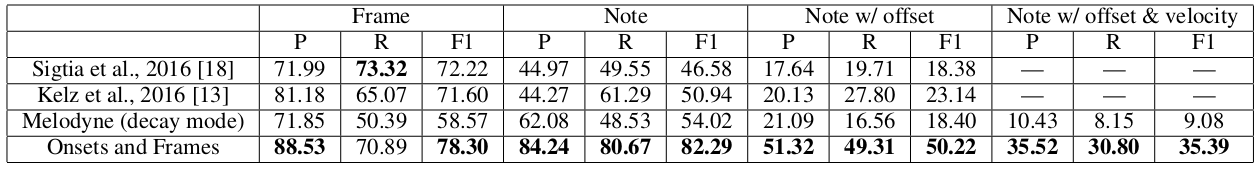
\includegraphics[width=\linewidth]
    {./statics/hawthorne2017onsets_results.png}
    \caption{مقایسه عملکرد مدل \cite{hawthorne2017onsets} با کارهای قبلی}
\end{figure}

همچنین در شکلی که در ادامه آمده نمونه‌ای از ورودی مدل و مقایسه خروجی آن با مقادیر
برای یک نمونه تصادفی نمایش داده شده است.

\begin{figure}
    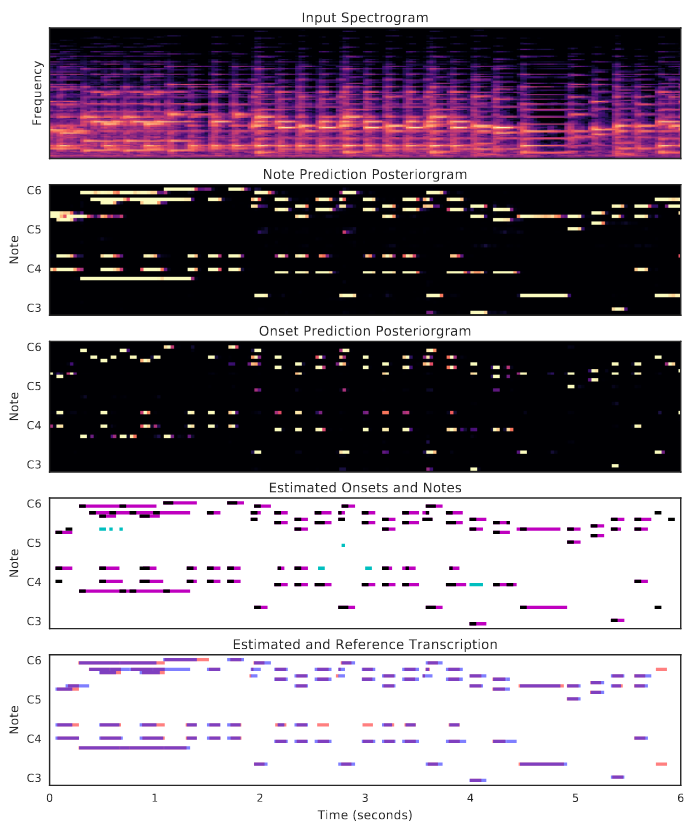
\includegraphics[width=\linewidth]
    {./statics/hawthorne2017onsets_spectorgrams.png}
    \caption{نمونه‌ای از ورودی و خروجی مدل \cite{hawthorne2017onsets}}
\end{figure}

\section{بررسی مرجع \cite{hawthorne2018enabling}}
با وجود این که هدف اصلی این مقاله تولید موسیقی است و در نگاه اول زیاد ارتباطی
با موضوع پایان‌نامه ندارد ولی شکلی که این قطعات جدید تولید می‌شوند کاملا با مسئله
آوانویسی گفتار مرتبط است. این مدل قطعات جدید را در ۳ مرحله تولید می‌کند. قدم اول
آوانویسی قطعات موجود در دیتاست است. سپس بر روی این نمایش‌های نمادین تولید شده
مدلی موسیقیایی تولید می‌شود. با نمونه گیری از این مدل می‌توان حالت نمادین قطعات
جدید را تولید کرد. در نهایت این قطعات تولید شده توسط مدلی دیگر به فرم صوتی باز
گردادنده می‌شوند. همچنین دیتاست جدیدی در این مقاله معرفی شده است که تلاش کرده است
مشکلات دیتاست‌های قبلی، مانند
MAPS
را رفع کردند.

\subsection{مدل آوانویسی}
مدلی که این مقاله برای آوانویسی استفاده کرده است بر اساس مدل استفاده شده در
\cite{hawthorne2017onsets}
است. استفاده از دیتاست
MAESTRO
بجای دیتاست
MAPS
برای آموزش شبکه، باعث دقت بالاتری شده است. همچنین وجود قسمت اعتبارسنجی در این
مقاله کمک کرده است تا جست‌وجوی ابر مقدارها ساده‌تر شده و در نتیجه دقت مدل مجددا
افزایش پیدا کند.

همچنین به علتی این که دیتاست جدید، بسیار بزرگ‌تر است، اندازه لایه
\lr{bidirectional LSTM}
از ۱۲۸ نرون به ۲۵۶ افزایش یافت. همچنین تعداد فیلترها در شبکه عصبی پیچشی از
۳۲-۳۲-۶۴
لایه به
۴۸-۴۸-۹۶
بایه افزایش یافته است. همچنین تغیرات کوچک دیگری در بخش‌های دیگر داده شده است.
به صورت کلی این مقاله معتقد است وقتی که اندازه دیتاست آموزشی افزایش یابد بهترین
راه برای افزایش عملکرد مدل، بزرگ‌تر کردن آن است.

همچنین این مقاله از تشدید داده برای افزایش مصنوعی حجم داده استفاده کرد است.
به این صورت که در زمان آموزش مدل هر نمونه از داده آموزشی با استفاده از ابزار
\lr{SoX}
دستکاری می‌شود. این دستکاری که به صورت تصادفی انجام می‌شود باعث می‌شود که مدل زمان
آموزش یک قطعه را هیچ گاه عینا دوبار نبیند در نتیجه قابلیت تعمیم آن افزایش یابد.
در شکل زیر مقدار هر یک از این تغییرات آمده است. نکته قابل توجه این است که
برخلاف انتظار زمانی که تشدید دیتا فعال باشد، دقت یادگیری بر روی دیتاست
MAESTRO
مقداری کاهش پیدا می‌کند. این تغییر در شکل زیر مشخص است.

\begin{figure}
    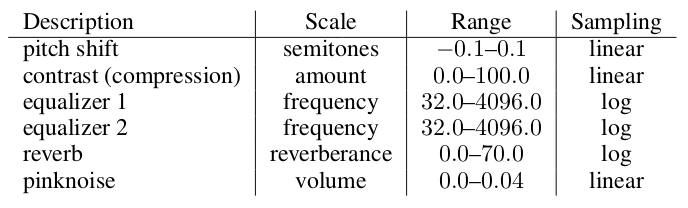
\includegraphics[width=\linewidth]
    {./statics/hawthorne2018enabling_augmentaion_parameters.png}
    \caption{لیست تبدیل‌های استفاده شده در \cite{hawthorne2018enabling}}
\end{figure}

\begin{figure}
    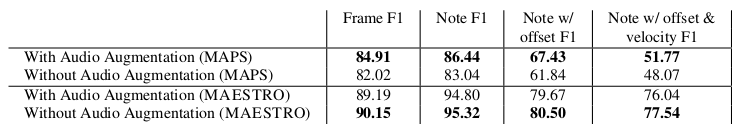
\includegraphics[width=\linewidth]
    {./statics/hawthorne2018enabling_augmentaion_results.png}
    \caption{نتایج حاصل از تشدید داده در \cite{hawthorne2018enabling}}
\end{figure}

همچنین وقتی مدل با استفاده از دیتاست
MAESTRO
آموزش داده شد، عملکرد مدل حتی برای دیتاست
MAPS
نیز مجددا افزایش یافت، که در شکل زیر این مقداری مشخص است.

\begin{figure}
    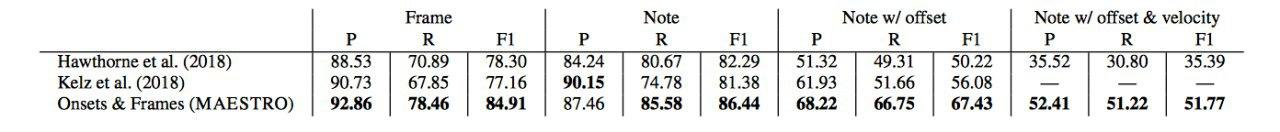
\includegraphics[width=\linewidth]
    {./statics/hawthorne2018enabling_maps_results.jpg}
    \caption{دقت مدل‌های مختلف بر دیتاست MAPS \cite{hawthorne2018enabling}}
\end{figure}

\begin{figure}
    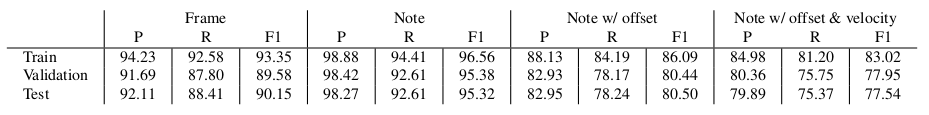
\includegraphics[width=\linewidth]
    {./statics/hawthorne2018enabling_maestro_results.png}
    \caption{دقت به دست آمده بر روی MAESTRO در \cite{hawthorne2018enabling}}
\end{figure}